\documentclass[a4paper,12pt]{article}

\usepackage{isolatin1}
\usepackage{verbatim}
\usepackage{palatino}
\usepackage{wrapfig}
\usepackage{color}
\usepackage{xspace}
\usepackage{graphicx}
\usepackage{hyperref}

\usepackage[nofancy,today]{rcsinfo}

%%% -- Set rcs info -----------------------------------------------------

\rcsInfo $Id$ 

%%% -- Useful macros ----------------------------------------------------

%% The code environment typesets its contents verbatim.
\def\code{\verbatim}
\def\endcode{\endverbatim}
%% Same typesetting as code, but different name; this is
%% for code you do not want to show up in literal scripts. 
%% (i.e. the code with syntax errors in it :-)
\def\xcode{\verbatim}
\def\endxcode{\endverbatim}
%% Code snippets in the text:
% \def\codetxt{\textcolor{codecol}\verb} %% hmm...
% \let\MMTextTT=\texttt{}
% \renewcommand{\texttt}[1]{\textcolor{codecol}{\MMTextTT{#1}}}


%%% -- Configuration ----------------------------------------------------

\hyperbaseurl{file:///home/cxl/src/uni/htk/doc/hdoc/}

%
% Colour setup (to come?)
%

\definecolor{linkcol}{rgb}{0.1,0.1,0.4} % dark blue

\ifx\hypersetup\undefined\relax\else
 \hypersetup{%
    %breaklinks=true,
    colorlinks=true,
    %hyperindex=true,
    pdfpagemode=None,
    linkcolor=linkcol,
    citecolor=linkcol,
    %plainpages=false,
    hypertexnames=false
 }
\fi

%
% Layout
%

% no parindent
\setlength{\parindent}{0pt}
\setlength{\parskip}{1ex}  

% wider page
\addtolength{\textheight}{1cm}
\addtolength{\textwidth}{2cm}
\addtolength{\evensidemargin}{-1cm} 
\addtolength{\oddsidemargin}{-1cm}
                                                   

\title{A Short Introduction to \HTk \\
  Graphical User Interfaces for Haskell}

\author{Christoph L�th \\ FB 3 -- Mathematik und Informatik,
  Universit�t Bremen}

\newcommand{\HTk}{\textsc{HTk}\xspace}

\newcommand{\ToBeDone}[1]{\textbf{TBD: #1}}



\begin{document}

\ifx\pdfoutput\undefined\maketitle
\else
\includegraphics[width=\textwidth]{img/intro-title}\fi

\begin{abstract}
  This paper introduces the basics of \HTk, a toolkit to build
  graphical user interfaces in Haskell. \HTk{} is an
  encapsulation of Tcl/Tk \cite{Ousterhout,Welch}, but we will not
  assume any previous knowledge of Tcl/Tk. The article is meant as a
  rough guide and introduction to the structure of \HTk. It is not
  meant as a complete reference manual; Rather, it should give readers
  enough information and background to get them started on their first
  \HTk programs, to know which parts of \HTk might be potentially useful
  in the applications they have in mind, what is feasible to build
  with \HTk, and finally to enable them to find further
  information quickly in the reference material.
\end{abstract}

\vfill{}
{\scriptsize\raggedleft{Source: \rcsInfoFile, 
  Revision \rcsInfoRevision{} of \rcsInfoDate}\par{}}

\newpage

\tableofcontents{}

\subsection*{How to Read This Document}
For maximum benefit, you should read this text in its PDF incarnation,
and enable your acrobat reader to display weblinks (menu
\texttt{File}, submenu \texttt{Preferences}, submenu
\texttt{Weblink}). If you have configured \HTk correctly, then the
hyperlinks in this document should display the corresponding online
reference material; \href{index.html}{this should take you to the
  index page}. The online reference material can also be found in
\texttt{htk/doc/hdoc}.

\section{Getting Started}

\subsection{Basics}

When we design and implement a graphical user interface, we have to
take two aspects into account: the \emph{static} aspect, which
specifies its appearance (which buttons to place where, what menues to
display, etc.), and the \emph{dynamic} aspect, which specifies its
behaviour in reaction to the user's actions. The two can be
interlinked: as a reaction to the user's action, the graphical user
interface may change its appearance.

In \HTk, these two aspects are modelled by \emph{monads}. The static
aspect is modelled in the \texttt{IO} monad, where all of Haskell's
external interactions takes place. The dynamic aspect is modelled by
\emph{events}. For a more complete description of events, we refer to
\cite{ger:Events}, but for the time being, events are an abstract datatype
with three main operations:

\begin{itemize}
\item The central operation is \emph{synchronisation}
\begin{verbatim}
sync :: Event a-> IO a
\end{verbatim}
which holds the current thread until an event of type \texttt{Event a}
occurs.  The basic events will be user interactions, such as clicking
a button. 
\item  The \emph{sequencing} operator
\begin{verbatim}
(>>>=) :: Event a-> (a-> IO b)-> Event b
\end{verbatim}
attaches an IO action to an event; if we synchronize on this event,
the IO action will be performed after the event occurs. 
\item Finally, the \emph{always} operator turns an IO action into an event:
\begin{verbatim}
always :: IO a-> Event a
\end{verbatim}
\end{itemize}
Events form a monad, with monad composition given by \texttt{>>>=} and
\texttt{always}. The monad composition corresponds to event sequencing;
if we synchronise on an event composed from simple events, we wait for
each of them in turn. By composing events in this way, fairly complex
behaviours can be modelled in a single event.

That the dynamic behaviour is not modelled with \texttt{IO} actions
directly reflects the fact that user interaction in a graphical user
interface is different from other forms of I/O, because it happens
asynchronously.

Further, events allow the user interface to be concurrent in a natural
and controlled way, leading to a reasonable and still tractable degree
of concurrency; the function
\begin{verbatim}
spawnEvent :: Event () -> IO (IO ())
\end{verbatim}
spawns a concurrent thread which syncronises on the given event. The
\texttt{IO} action returned kills the concurrent thread.

\input{Mainsimple1.lhs}

\input{Mainsimple2.lhs}

\subsection{Structure of this Paper}

The rest of this paper is organized as follows: we will first explain
the organization of the datatypes modelling the static behaviour of
the graphical user interface. In Section~\ref{sec:events}, we will
describe events and in particular how to generate them from user
input. After this, we will embark on a guided tour through \HTk's
widgets (Sect.~\ref{sec:basic-widgets} to
Sect.~\ref{sec:tix-widgets}), covering basic widgets, menues, editors,
canvasses, windows and tix widgets, finishing off with an overview of
\HTk's toolkit.

\section{Elements of \HTk}

In general, \HTk has a couple of abstract datatypes used to model
elements of the graphical user interface, such as buttons, menues,
short text fields, longer texts, and so on. Recall from
Section~\ref{ssec:ex1} above that there is an abstract datatype
\texttt{Button}, elements of which are created with the function
\begin{xcode}
newButton :: Container par=> par-> [Config Button]-> IO Button
\end{xcode}
This takes a parent GUI element, and a list of configurations as
parameter. We will first examine the class \texttt{Container}, which
models the GUI element hierarchy, and then the configurations,
followed by resources such as fonts and colours. At the end of this
section, we explain packing.

\subsection{The GUI element hierarchy and the \texttt{Container} class.}

The class \href{Packer.html#Container}{\texttt{Container}} designates
GUI elements into which other GUI elements may be packed.

Instances of \texttt{Container} include \texttt{Toplevel} (windows),
\texttt{HTk} (Tk's root window), \texttt{Frame}, and furthermore
\texttt{Canvas}, and \texttt{Editor} (and a few Tix widgets).

The class \texttt{Container} is \emph{abstract} --- it has no class
functions, and only serves to structure the code. Abstract classes are
used frequently in \HTk to impose a typing discipline onto Tk's untyped
GUI element structure, with the benefit that type checking can prevent
run time errors.

\subsection{Configurations}

Above, the text of the button was set with a \emph{configuration
  option}. Configuration options determine various attributes of a
widget. They can be given at the time of creation, or changed later
on. In general, the configuration type is just a type
synonym\footnote{Type synonyms 
  like that in class confusions confuse Hdoc, which is why they appear
  expanded at various places of \HTk's source code--- just in case you
  happen to browse it, which you are more than welcome to.}
\begin{xcode}
type Config w = w -> IO w
\end{xcode}
As seen above, configurations can be given at the time of creation, or
later on. In the latter case, the helpful \texttt{(\#)} operator
provides useful syntactic sugar:
\begin{xcode}
( # ) :: a -> (a -> b) -> b
o # f = f o  
\end{xcode}
Some configurations are only supported by one particular widget, and
thus are a simple monomorphic function. However, most configurations
are supported by many, but not all widgets, and each configuration by
different ones, and this behaviour is modelled in \HTk by type
classes. Common configuration classes can be found in the module
\href{Configuration.html}{\texttt{Configuration}}. For example, the
text configuration is given by this class:
\begin{xcode}
class (GUIObject w, GUIValue v) => HasText w v where
  text :: HasText w v => v -> Config w
  getText :: HasText w v => w -> IO v
\end{xcode}
The class \texttt{GUIObject w} is one of \HTk's most basic classes.
Its instances are widgets and other interface elements we will
encounter later (canvas items, text tags, windows). \texttt{GUIValue
  v} is another basic class, the instances of which are all basic
datatypes which can be communicated to Tk: \texttt{Int},
\texttt{Double}, \texttt{Bool}, \texttt{String} and \texttt{[String]}.
Now, all widgets can be configured with a text are instances of the
class \texttt{HasText}, such as \texttt{Button}.


\subsection{The class \texttt{Destroyable}}
\label{ssec:destroyable}

The class \texttt{Destroyable a} has the main class function
\begin{xcode}
  destroy :: a-> IO ()
\end{xcode}
which when called will destroy its argument. All GUI elements are
instances of this class, and calling the destroy function will remove
them from the screen. In particular,  destroying the return
value of \texttt{initHTk} will close all windows opened by the program
(i.e. remove the whole GUI). 

\subsection{Concurrency and the class \texttt{Synchronize}}

The class \texttt{Synchronize a}, with its main and only class
function
\begin{xcode}
  synchronize a :: a-> IO b-> IO b
\end{xcode}
describes a \emph{monitor}, like the synonymous method in the
programming language \textsc{Java} \cite{ArnoldGosling}. All GUI
elements are instances of this class. It allows convenient handling of
concurrency--- if two IO actions must not interleave, you synchronize
them on any one GUI element, typically the one generating the event
which the function calling the two IO actions is bound to.


\subsection{Resources}

Resources are auxiliary datatypes modelling distances, colours, fonts,
pictures and cursor shapes.

\subsubsection{Geometry}

The abstract data type \texttt{Distance}, implemented in the module
\href{Geometry.html}{\texttt{Geometry}}, represents distances in \HTk.
Distances can be specified in \texttt{cm}, \texttt{mm}, \texttt{ic}
(inches) and \texttt{pp} (points), with functions  \texttt{cm:: Int->
  Distance} etc. Moreover, \texttt{Distance} is an instance of
\texttt{Num}, so we can specify the distance 3 (meaning 3 pixels)
directly. 

\subsubsection{Colours}

The abstract data type \texttt{Colour}, implemented in the module
\href{Geometry.html}{\texttt{Geometry}}, represents colours in
HTk. Just like distances, the type itself is abstract, but unlike
distances, there is a class \texttt{ColourDesignator} allowing
colours to be specified in a flexible manner by overloading. Functions
expecting a colour as an argument take any instance of
\texttt{ColourDesignator} as argument, such as 
\begin{xcode}
background :: (ColourDesignator c, HasColour w) => c -> Config w 
foreground :: (ColourDesignator c, HasColour w) => c -> Config w   
\end{xcode}
which set the background or foreground of any interface element which
has a colour (nearly all). Its main instances are:
\begin{xcode}
instance ColourDesignator [Char]
instance ColourDesignator (Int, Int, Int)
instance ColourDesignator (Double, Double, Double)  
\end{xcode}
The strings are named colours (\texttt{red}, \texttt{white},
\texttt{black}, etc.), the tuples are RGB values. (The functions of
the type classes \texttt{HasColour} and \texttt{ColourDesignator} are
for HTk's internal consumption only, but annoyingly appear all over
the documentation.)

\subsubsection{Fonts}

Fonts are implemented in the module
\href{Font.html}{\texttt{Font}}. The datatype \texttt{Font} represents
the specification of exactly one font in the usual (X-style) way,
by giving a family, slant, spacing, width and weight. For example, the
family is given by 
\begin{xcode}
data FontFamily = Lucida | Times | Helvetica 
                | Courier | Symbol | Other String  
\end{xcode}
where the five enumerated types are available on most systems. With
\texttt{Other}, you can directly give a more exotic family such as
\texttt{clearlyu alternate glyphs}. 

Just like with colours, there is a class
\href{Font.html#Font.FontDesignator}{\texttt{FontDesignator}}, the
instances of which give ways of describing fonts, such as the following:
\begin{xcode}
instance FontDesignator FontFamily 
instance FontDesignator (FontFamily,Int) 
instance FontDesignator (FontFamily,FontWeight,Int) 
instance FontDesignator (FontFamily,FontSlant,Int) 
instance FontDesignator String 
instance FontDesignator XFont 
\end{xcode}
The first three allows fonts to be specified by the font family, plus
the size, plus the weight or the slant, respectively; the second from
last allows an X-style string
(e.g.
\texttt{-adobe-courier-bold-o-normal-*-14-*-*-*-*-*-iso8859-*-}), and
the last an X-style specification as an abstract datatype. 

Be warned that fonts are, in principle, not very portable under X,
since the available fonts are determined by the fonts of the X server
the programm is running on. It is best to stick to well-known font
families such as the above, and usual sizes. (So, no \texttt{clearlyu
  alternate glyphs} in 144 pixels.)

\subsubsection{Images and Bitmaps}

\href{Images.html}{Images} are representation of pictures, from wee
icons to screen-filling murals. \HTk's images are what in Tk is called
a photo. An image is created with the function
\begin{xcode}
newImage :: [Config Image] -> IO Image  
\end{xcode}
Once created, an image can be attached (via the \texttt{photo}
configuration, class \texttt{HasPhoto}) to labels, buttons, and canvas
items. The configuration gives the image's data, either via the
\texttt{filename} configuration, where a file is specified which
contains the image data, or via the \texttt{imgData} configuration,
which passes the data directly as Base64 encoded string. (You can use
e.g.  the \texttt{mimencode(1)} utility to produce such a string.) As
can be seen from the \texttt{Format} datatype, \HTk{} supports GIF,
PPM and PGM formats. The latter method of giving the image data is
preferable, since it makes the compiled executable independent of
image data files; if you pass a filename, you need to make sure that
the image file is to be found at that path during the \emph{runtime}
of the program!

\href{BitMap.html}{Bitmaps} have a foreground and a background. The
difference between images and bitmaps is that bitmaps are more
versatile, e.g. you can change the foreground and background, but only
have two colours. There is also a number of predefined bitmaps
(\texttt{Hourglass, Questhead}, etc.) Apart from that, bitmaps are
quite boring.

\subsubsection{Cursors} 

Any widget can change the shape of the cursor, i.e. the shape
displayed by the cursor while over this widget, by using the
\href{BaseClasses.html#BaseClasses.cursor}{\texttt{cursor}}
configuration. The class \texttt{CursorDesignator} from the module
\href{Cursor.html}{Cursor} module allows cursors to be specified in an
overloaded way (like colours and fonts). The simplest way to get a cursor is to
avail yourself of some of the predefined ones (at least under X
windows), but you can build your own cursor by giving a bitmap, a
mask, and colours.


\subsection{Packing}

\label{sec:packing}

As mentioned above, after widgets have been created (with e.g.
\texttt{newButton}), they will not be displayed just yet; this only happens
after they have been packed. One can use this effect by first creating
lots of widgets, and then packing them in one go, lessening the
unpleasant flicker effect occuring when the GUI is built one interface
at a time. To minimize the flickering further, use the function
\begin{xcode}
delayWish :: IO a-> IO a
\end{xcode}
which delays all \texttt{Tk} commands in the argument, and performs
them at once. The argument then consists of a sequence of
\texttt{pack} commands. Unfortunately, the flickering effect cannot be
totally eliminated.

Packing in particular determines the visual layout of the GUI by the
order in which the widgets are packed, and by packing options. Tk's
know different packing algorithms (or \emph{geometry managers}, in Tk
parlance); of these, \HTk supports the pack geometry manager, and the grid
geometry manager. The third, the place geometry manager, could easily
be added, if you are so inclined.

\subsubsection{The Standard Packer}

The behaviour of the standard packer is easily explained, and hard to
understand. Widgets are packed with the function
\begin{xcode}
pack::Widget w => w -> [PackOption] -> IO ()  
\end{xcode}

The datatype
\href{PackOptions.html#PackOptions.PackOption}{PackOption}
is defined as 
\begin{xcode}
data PackOption = Side SideSpec  | Fill FillSpec 
                | Expand Toggle  | Anchor Anchor
                | IPadX Distance | IPadY Distance
                | PadX Distance  | PadY Distance
\end{xcode}
The first two constructors are most important here. The
\href{PackOptions.html#PackOptions.SideSpec}{SideSpec} specifies where
the widget is packed (top, bottom, left, right), and
\href{PackOptions.html#PackOptions.FillSpec}{FillSpec} specifies in
which direction it expands to fill the available space.  Bear in mind
that widgets are packed as tight as possible, and that once packed,
they are never repacked, moved or resized. That is, if e.g. a widget
is packed against the top, it will sit in the middle (if no
\texttt{Fill X} is specified), and will not move if a widget is packed
against the right-hand side, although the window may be increased in
size to make a new widget fit.

\texttt{Expand} just means that the widget expands when the containing
element is expanded (i.e. the window is resized), and \texttt{Anchor}
specifies a gravity (a side to which the widgets stick). The rest
create a padding border around the widget in various directions.

It is quite normal that most of the time the arrangement of the
widgets will not look
like intended, and you will need to use frame widgets (see
Section~\ref{ssec:frames}).

\subsubsection{The Grid Packer}

The grid packer divides the container widget into a grid, and allows
placement of widgets relative to that grid. To pack a single widget
use the following function:
\begin{xcode}
grid :: Widget w => w -> [GridPackOption] -> IO ()
\end{xcode}

The datatype
\href{GridPackOptions.html#GridPackOptions.GridPackOption}
{\texttt{GridPackOptions}} specifies the packing options for the grid
packer.

Within the same container you cannot use different packing
algorithms. The first widget packed into a container defines the
packing for this container.

\section{Events}

\label{sec:events}

In general, events are an abstract datatype for communication and
synchronisation, much in the spirit of process algebras such as CCS
\cite{Milner:CommunicationConcurrency}, CSP \cite{Roscoe} or
the $\pi$ calculus \cite{Milner:PiCalculus}. Here, an 
\href{Events.html}{\texttt{Event}} is
an abstract datatype with operations such as \texttt{sync},
\texttt{+>} and \texttt{>>>=}, which additionally form a monad; we
refer to \cite{ger:Events} for more information. 

In \HTk, basic events arise from user interactions by means of the
\emph{bind} commands. By binding a user interaction (such as clicking
a button), we set it up to produce an event, on which we can
synchronise and thus produce a reaction to the user's action. We can
then use the event operators to build more complex events with these
basic events.

One important caveat here is that once you set up a binding, you
\emph{must} eventually \emph{synchronise} on the resulting events, since
otherwise the unused events will pile up and result in a memory
leak.

Bindings are generated by calling one of \texttt{clicked},
\texttt{bindSimple} and \texttt{bind}, where \texttt{bind} is most
flexible, as can be seen by its complex type.

\subsection{Simple Clicks}
\label{ssec:teenage-clicks}

Simple interface elements such as buttons and menu entries which
  are instances of the class
  \href{HTk.html#HTk.HasCommand}{\texttt{HasCommand}}. For these, we
  have a function
\begin{xcode}    
clicked :: HasCommand w => w -> IO (Event ())
\end{xcode} 
The event here occurs when the element is clicked. The event does
not have any additional information --- a click is just a click, after
all.

\subsection{Simple Binds}
For all GUI elements, the function
  \href{HTk.html#HTk.bindSimple}{\texttt{bindSimple}} provides a
  simple way of binding. Its arguments are the GUI element concerned,
  and a specification of the kind of events we are interested in:
\begin{xcode}    
bindSimple::GUIObject wid => wid -> WishEventType 
                                 -> IO (Event (), IO ())
\end{xcode}
\href{HTk.html#HTk.WishEventType}{\texttt{WishEventType}} is an
algebraic data type describing the kind of event we would like to bind
to, much along the lines of Tk's events:
\begin{xcode}
data WishEventType =
   ButtonPress (Maybe BNo) | ButtonRelease (Maybe BNo) |
   Motion |
   Enter  | Leave | 
   KeyPress (Maybe KeySym) | KeyRelease (Maybe KeySym)|
   Activate | Circulate | Colormap | Configure | Deactivate |
   Destroy | Expose | FocusIn | FocusOut | Gravity |
   Map | Property | Reparent | Unmap |
   Visibility deriving (Show,Eq,Ord)
\end{xcode}
Each constructor corresponds to a different event, such as
\begin{itemize}
\item mouse buttons pressed and released (\texttt{ButtonPress (Maybe
    BNo)}, \texttt{ButtonRelease (Maybe BNo)}, where \texttt{BNo} is
  just \texttt{Int}),
\item mouse movements (\texttt{Motion}),
\item the mouse entering or leaving a GUI element (\texttt{Enter},
  \texttt{Leave}),
\item keys pressed or release (\texttt{KeyPress (Maybe KeySym)},
  \texttt{KeyRelease (Maybe KeySym)}),
\item and various window events (\texttt{Map}, \texttt{Unmap},
  \texttt{Expose}, \texttt{Activate},\ldots).
\end{itemize}
Note that not every GUI element can generate every event. Obviously,
only windows can generate window events, but more subtly, only entry
widgets, editor widgets and toplevels (i.e. windows) can generate
\texttt{Key} events.

The return value of \texttt{bind} is an event, and an IO action which
unbinds the event. You should use this action if you are not
interested in the event anymore (i.e. it will not be synchronised on
anymore), otherwise there will be a memory leak.

\subsection{Full Bindings}

In fact, \texttt{bind} is only a simplified version of the
  function \href{HTk.html#HTk.bind}{\texttt{bind}}
\begin{xcode}
bind::GUIObject wid => wid -> [WishEvent] 
                       -> IO (Event EventInfo, IO ())
data WishEvent = WishEvent [WishEventModifier] 
                           WishEventType
\end{xcode}
where
\href{HTk.html#HTk.WishEventModifier}{\texttt{WishEventModifier}}
desribes possible event modifiers such as \texttt{Shift},
\texttt{Alt}, \texttt{Meta} (corresponding to the Shift, Alt or Meta
key being held), \texttt{Button1}, \ldots, \texttt{Button5}
(corresponding to mouse button 1 thru 5 being pressed) or \texttt{Double} and
\texttt{Triple}. Again, not all combinations of modifiers and events
make sense; for example, double and triple pertain to mouse button
presses, and modifying a mouse button press with a different button is
not really helpful. Note that the argument of bind is a list of
events, meaning of course that each of the events generates in event
(not their combination).

Here, the first component of the return value is an event of
\texttt{EventInfo}, which is a labelled record as
follows:\footnote{Unfortunately, HDoc chokes on the relevant part of
  the source right now, so this is not in the reference manual.}
\begin{xcode}
data EventInfo = EventInfo { x :: Distance,
                             y :: Distance,
                             xRoot :: Distance,
                             yRoot :: Distance,
                             button :: Int }
\end{xcode}
The information here is the x and y component of the mouse position,
both relative to the window in which the event occurs, and the root
window (i.e. the screen), and the button being pressed. 

\section{Basic Widgets}
\label{sec:basic-widgets}

In the following sections, we give a brief tour around \HTk's widgets.
We have simple widgets which are explained in short sentences of words
with less than three syllables, menues, text widgets, and canvasses,
which require a slightly longer explanation.

There are more widgets: if you can use Tix (an enhance version of
Tcl/Tk; you should use it anyway, it
looks slightly less clunky than plain Tcl/Tk), there are the useful
tab and pane widgets. And because \HTk is an abstraction on top of Tk,
there are a variety of so-called \emph{mega-widgets} which are
implemented in Haskell; these can be found in the toolkit
(Sect.~\ref{sec:toolkit}).

\subsection{Frames}

\label{ssec:frames}

A \href{Frame.html}{frame} is just an invisible container into which
we can pack other widgets, grouping them together. The use of frames
is in packing: the grouping is necessary most of the time to achieve
the desired layout with the standard packer.

Moreover, when using a frame, we can use a different packer (see
Sect.~\ref{sec:packing}) than in the parent widget; for example, we
can use the grid packer inside a window using the standard packer.

\subsection{Boxes}
  
  \href{Box.html}{Boxes} are mega-widgets, implemented using frames.
  They allow simple horizontal or vertical packing (widgets are placed
  in the box side by side or on top of each other), and be flexible or
  rigid (expand when the parent window is resized, or not); e.g.
  \texttt{newVBox} creates a rigid box with vertical packing, and
  \texttt{newHFBox} creates a flexible box with horizontal packing.

\subsection{Buttons}

  A \href{Button.html}{button} is a simple widget which can be
  clicked. Buttons can have bitmaps, images (class \texttt{HasPhoto}),
  or text as labels. 

\subsection{Labels and Messages}
  
  A \href{Label.html}{label} is a simple widget for text, bitmaps or
  images. \href{Message.html}{Messages} are slightly more
  sophisticated widgets for longer text messages; messages linebreak
  the text. For both, the font of the text (class \texttt{HasFont})
  and the justification (class \texttt{HasJustified}) can be
  specified. The \texttt{aspect} configuration (for messages only)
  specifies the width of the text as a percentage of the height; so
  \texttt{aspect 200} gives a message twice as wide as high.

\input{Mainentry.lhs} %% Entry widgets.

\input{Mainlist.lhs} %% Scrollbars, List boxes.

\input{Mainmenu.lhs} %% Menues

\section{The Editor}

\label{sec:textwidget}

An editor (also called a text widget) is a very flexible and powerful
widget to display and edit texts. As opposed to labels and messages,
is scrollable (i.e. an instance of class
\href{ScrollBar.html#ScrollBar.HasScroller}{HasScroller}), but its
chief difference to labels and messages are that it can be
\emph{edited} and has \emph{text tags}, which make into one of Tk's
most powerful widgets. 

Editors are created with \texttt{newEditor}. The datatype
\texttt{Editor} is monomorphic, but editors have a value (their
textual content), and are thus members of the class \texttt{HasValue}.

Besides the usual, editors provide configurations to
\begin{itemize}
\item set the spacing with the
  methods of the class
  \href{Editor.HasLineSpacing}{\texttt{HasLineSpacing}},
\item set the wrap mode (character, word, or no wrap) with the function
  \href{Editor.html#Editor.wrap}{\texttt{wrap}},
\item and set tabulators with the class
  \href{Editor.html#Editor.HasTabulators}{\texttt{HasTabulators}}. 
  \ToBeDone{How are tabulators specified?}
\end{itemize}

Text can be appended (\texttt{appendText}) or inserted at a specified
position into the editor with the function
\href{Editor.html#Editor.insertText}{\texttt{insertText}}: 
\begin{xcode}
insertText::(HasIndex Editor i BaseIndex, GUIValue a) => 
            Editor -> i -> a -> IO ()
\end{xcode}
The position where the text is inserted is specified by the class
\texttt{HasIndex}.

\subsection{Indices}

\label{ssec:indices}

The type \texttt{BaseIndex} also models indices into list boxes, entry
widgets \textit{etc.}, but for editors only the constructor
\texttt{IndexPos} is important:
\begin{xcode}
data BaseIndex =
  IndexNo Int | IndexPos Position | IndexText String 
\end{xcode}
The class \texttt{HasIndex} models which way of indexing a position
inside a widget is valid.\footnote{From an abstract point of view, the
  type class is unfortunate, since the last type parameter is only for
  internal consumption; it models the so-called base index of the
  widget, i.e. the type into which other ways of indexing will have to
  be translated. As a user, you can just disregard the last parameter
  of the class.} For text widgets, we have
\begin{xcode}
instance HasIndex Editor BaseIndex BaseIndex  
\end{xcode}
so we can just specify the index as a position (i.e. a row and column
number, starting from 0), but we can also specify the index by the constant
\texttt{EndOfText} (only constructor of the data type
\texttt{EndOfText}), or by its screen coordinates (\texttt{Pixels}),
or by \emph{modifying} one of the other indices:
\begin{xcode}
instance HasIndex Editor EndOfText BaseIndex
instance HasIndex Editor Pixels BaseIndex
instance HasIndex Editor i BaseIndex => 
         HasIndex Editor (i, [IndexModifier]) BaseIndex
instance HasIndex Editor i BaseIndex => 
         HasIndex Editor (i, IndexModifier) BaseIndex  
\end{xcode}

Index modifiers (only for editors) are modelled by type
\href{Editor.html#Editor.IndexModifier}{\texttt{IndexModifier}}, and
specify things like `three words forward', or a `one line
back'.

\subsection{Selections}

\label{ssec:selections}

In an editor (and an entry widget), text can be \emph{selected} by
marking it with the mouse button. Similarly, in list boxes, entries
can be selected. Abstractly, these kind of selections are modelled
with the selection type classes (module
\href{Selection.html}{\texttt{Selection}}). There are five classes, of
which \texttt{HasSelection}, \texttt{HasSelectionIndex} and
\texttt{HasSelectionIndexRang} let you set the selection, and
\texttt{HasSelectionBaseIndex} and \texttt{HasSelectionBaseIndexRange}
let you query the selection. The selected text, entries \textit{etc.}
are indexed with indices (see Sect.~\ref{ssec:indices}). The
\texttt{Range} classes have a pair of functions, which set or get the
start or end of the selection, respectively, whereas the
\texttt{HasSelectionIndex} and \texttt{HasSelectionBaseIndex} classes
get or set the selection as list of indices.

This selection is Tk-internal, and should not be confused with
selection as implemented by X Windows. This selection is handled by
the class \texttt{HasXSelection}. Its instances are entries and
editors. For those, Tk's selection can also be the X selection. The
module \href{XSelection.html}{\texttt{XSelection}} allows access to
the X selection (get the current selection, selecting wether widgets
export their selection etc.)


\subsection{Text Tags}

A text tag is a way of marking a specified section of the text. One
text tag can mark a list of ranges, which are specified by a start and
an end index: 
\begin{xcode}
createTextTag :: (HasIndex Editor i1 BaseIndex,
                  HasIndex Editor i2 BaseIndex) =>
                 Editor -> i1 -> i2 -> [Config TextTag] -> IO TextTag  
\end{xcode}
Once we have a text tag, we can \href{TextTag.html}{configure
 it}. It has a font, colour, cursor, justification, line spacing,
wrapping, tabulators and so on. Moreover, you can bind events to a
text tag, making it active; so when the mouse moves over the text, or
the user clicks the text, something exciting happens. This allows you
very easily to implement hypertext, references and so on. 

When you insert into an editor, the text tags are accommodated
appropriately; i.e. if you insert into the middle of a text tag,
then the end of the tag is moved accordingly.

\subsection{Editing}

As mentioned above, the editor's text can be edited, i.e. the user can
type text into the widget. This feature can be considered as a
conveniently set up set of key bindings (e.g. the key `a' is bound to
the function which inserts an `a' at the current cursor position). You
can switch off the editing behaviour with the function
\texttt{disable} from the class
\href{Configuration.html#Configuration.HasEnable}{\texttt{HasEnable}},
but be warned: \emph{You can only change the text of enabled editors!}
Trying to insert text into a disabled editor is one of the most common
Tk errors; it will not generate a run-time error but just silently
fail to change the text of the editor, leaving the programmer in
puzzled dismay.

The example \texttt{htk/examples/simple/Maintexttag.hs} shows what you
can do with text tags, and how to use them. The module
\texttt{MarkupText} from the toolkit allows a more abstract approach
to displaying text with differents fonts, hyperreferences and so on
(see Section~\ref{sec:toolkit} below). 

\subsection{Marks and More}

To keep track of positions within an editor, you can use marks (type
\href{Mark.html}{\texttt{Mark}}).\footnote{The first one to send us an
  email saying `Shouldn't this type have been renamed to Euro?'
  will be forcefed Perl scripts until his mind explodes into a regular
  expression. You have been warned. Other than that, we strongly
  encourage any comments about \HTk{} or this wee manual. Go on, send
  us that mail!} Essentially, you can put a mark
into an editor at a specified position (with \texttt{createMark}), and
query its position later (\texttt{getBaseIndex}). The gravity of the
mark specifies wether when text is inserted at the exact position of
the text, it should move to the left, or the right.

There's more you can do with an editor. For one, you can also insert
widgets into the text (this is called an \emph{embedded window}), with
the function 
\begin{xcode}
createEmbeddedTextWin :: (HasIndex Editor i BaseIndex, Widget w) =>
                         Editor -> i -> w ->
                         [Config EmbeddedTextWin] -> IO EmbeddedTextWin
\end{xcode}
so you can have buttons, entries, and even another editor inside an
editor (see the module \href{EmbeddedTextWin.html}{\texttt{EmbeddedTextWin}}).

Further, you can search the text inside an editor (with the
\texttt{search} function), read and write the contents to and from a
file, scroll the contents to a specific position, and much more as
found in the module \href{Editor.html}{\texttt{Editor}}.

\section{The Canvas Widget}
\label{sec:canvas-widget}

A canvas is a widget to draw on, i.e. we can put graphical objects on
it (lines, polygons, circles and ellipses, wee images, and even whole
widgets) at a specified position. A canvas is scrollable, so its
drawing area can be far larger than the displayed area.

The graphical objects on a canvas are called \emph{canvas items}. Just
like for widgets, the different kinds of canvas items are represented
by different types. Canvas items can be configured (but of course the
configurations are mostly different from widget configurations), and
we can bind events to them.

\subsection{Canvas Item Configurations}

The most important configurations, provided by all canvas items, are: 

\begin{itemize}
\item \texttt{HasCoords} sets or returns the coordinates of the canvas
  item on the canvas. Nearly all canvas items (except for lines) have
  a position (\texttt{HasPosition}), and many have a size
  (\texttt{HasSize}).
\item \texttt{FilledCanvasItem} allows to configure the filling
  colour, outline colour, stipple and width of the outline of the
  canvas item. Note that for some canvas item (e.g. lines), setting
  the outline does nothing, but setting the filling colour sets the
  colour of the item. A stipple, incidentally, is a bitmap mask used
  to draw the item. 
\end{itemize}

\subsection{Canvas Items} 

\begin{wrapfigure}[15]{r}{7cm}
  \begin{center}
    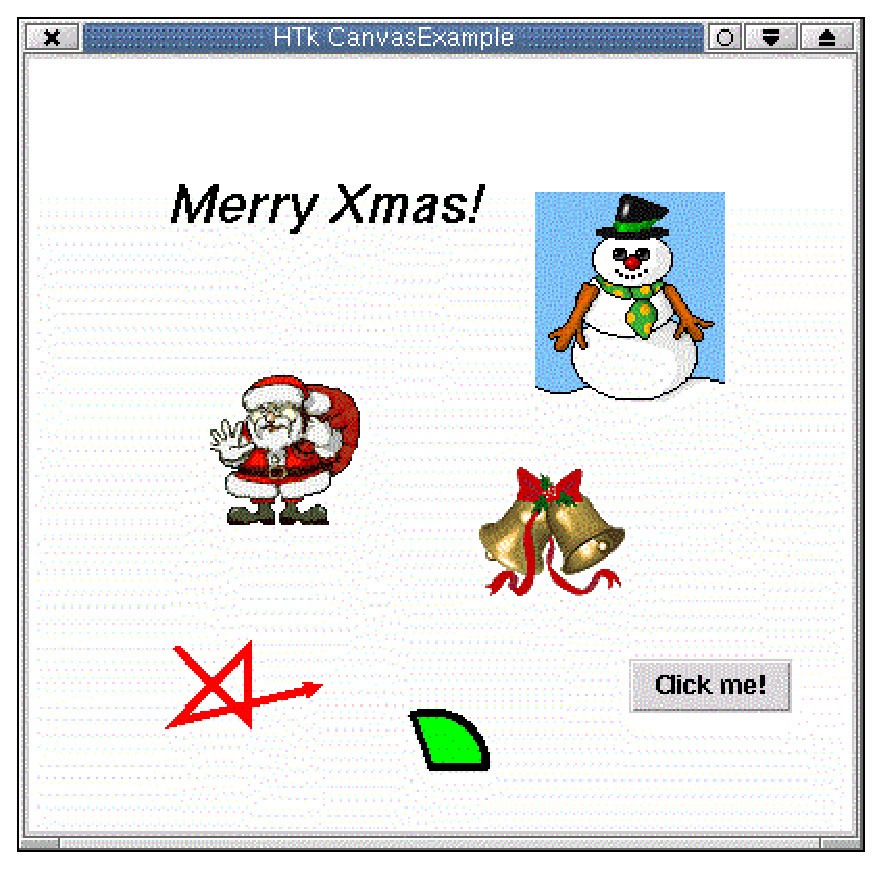
\includegraphics[width=6cm]{img/screenshot-canvas}    
  \end{center}
  \caption{Canvas items: 
    a text item, three image items, a line item, an arc and an
    embedded window (a button).}
  \label{fig:xmas-canvas}
\end{wrapfigure}
The following are the types of canvas items:

\begin{itemize}
\item \texttt{Arc}: a section of an oval, given by the start angle and
  the length (configurations \texttt{start} and \texttt{extent}).
\item \texttt{BitmapItem} and \texttt{ImageItem}: canvas items given
  by bitmaps and images. The image of an image item is set with the
  \texttt{HasPhoto} class, just like for some widgets.
\item \texttt{LineItem}: a line item is given by a list of two or more
  points, which define a list of line segments. The segments can be
  joined in various ways (with the \texttt{joinstyle} configuration),
  you can draw splines (class
  \href{CanvasItem.SegmentedCanvasItem}{\texttt{SegmentedCanvasItem}}), and put arrows on either (or both) ends (configurations \texttt{arrowshape} and \texttt{arrowstyle}). 
\item \texttt{Oval}: an oval is given by defining its \emph{bounding
    box}, i.e. the smallest rectangle enclosing it, using the classes
  \texttt{HasGeometry} or \texttt{HasPosition} and \texttt{HasSize}.
  If the bounding box is a square, the oval is a
  circle.\footnote{Except it usually won't \emph{look} like a circle
    on the screen, because on most screens pixels are
    rectangularly-shaped.}
\item \texttt{Polygon}: a polygon is given by a list of
  vertices. Strangely, one cannot configure the join style of the
  polygon, but you can configure splines.
\item \texttt{Rectangle}: a rectangle is given by two points. 
\item \texttt{TextItem}: a text item is a text, possibly consisting of
  more than one line. It is an instance of \texttt{HasFont}. (Note
  that \HTk{} curently does not support Tk's selection and insertion
  methods for text items; it should be easy to add, if you really
  require that.)
\item \texttt{EmbeddedCanvasWin}: an embedded canvas window is a
  widget embedded into a canvas. All instances of class
  \texttt{Widget} can be embedded into a canvas. Note that you don't
  need to pack embedded widgets; they appear as soon as the embedded
  canvas window is created.
\end{itemize}

\subsection{Canvas Tags}

A \emph{canvas tag} is a convenient way to refer
to canvas items. A canvas tag is an instance of the class
\texttt{CanvasItem} (but setting e.g. its filling colour will of
course have no effect). Canvas tags are in particular useful because
you can not only add canvas items explicitly to the tag, but also by
the so-called \textit{search specification}, so you can select the
canvas item closest to a given canvas location etc. 

For more on canvasses, see the examples under
\texttt{htk/examples/canvas}. \texttt{MainxmasCanvas.hs} (screenshot
Fig.~\ref{fig:xmas-canvas}) shows a variety of canvas items, and how
to set up a cheap and cheerful drag-and-drop.

\section{Windows}
\label{sec:windows}

What is commonly known as a window is called a \emph{toplevel} widget
in Tk and \HTk. They are created with a function 
\begin{xcode}
createToplevel :: [Config Toplevel] -> IO Toplevel
\end{xcode}
but (of course) they need not be packed, they just appear. Toplevels
are containers (instances of \texttt{Container}), so you can just pack
other widgets into them. They are closed by destroying them (see
Sect.~\ref{ssec:destroyable}). 

The familiar properties expected from a window are all in the class 
\texttt{Window} from module \href{Window.html}{\texttt{Window}}. Its
size can be configured either by classes \texttt{HasGeometry} or
\texttt{HasPosition} and \texttt{HasSize}, and its title by the class
\texttt{HasText}. The \texttt{screen} configuration sets the screen
the window appears on (the display in X windows speak).

In Tk, toplevels can have a menu attached which is the \emph{system
  menu} for this window. \HTk{} does not support this, but it should
be easy to do.

\subsection{Window Managers}

Windows are managed by the \emph{window manager}. It controls the size
and location of the windows appearing on the screen, trying to mediate
between the slew of applications vying for the user's attention. 

This means that even though the program can request a particular
geometry (i.e. size and location), it is not guaranteed to get it; in
particular, the window manager may decide to place the window
somewhere else entirely. 

\HTk{} does not support all of Tk's commands to communicate with the
window manager, but most of the important ones. These are the class
functions of the \texttt{Window} class, as mentioned above, and the
\href{Screen.html}{\texttt{Screen}} module, which allows you to query
the properties of the display (e.g. height and width).

\subsection{Focus}
\label{ssec:focus}

The \emph{focus} determines which window receives keyboard
events. It is managed by the window manager. Sometimes, it is
necessary for an application to \emph{grab the focus}, i.e. require
that all input go to this window before proceeding. For example when
implementing a window which asks the user to confirm a choice, you do
not want to user to start any other interaction, you want them to
answer the question. Such a window, which has to answered before the
program is allowed to proceed, is called \emph{modal}. 

Grabbing the focus is done with the functions \texttt{grabLocal} or
\texttt{grabGlobal} from the module
\href{Focus.html}{\texttt{Focus}}. A local grab means that the user
cannot interact with any other window from the same application; a
global grab means that the use cannot interact with any other
window. After grabbing the focus, you should return the grab with
\texttt{returnGrab}. 

Global grabs are dangerous, because if you forget to return the grab
(or even worse, your application crashes), the user is effectively
frozen out. On the other hand, for example when requiring sensitive
information such as passwords or credit card numbers, they are a good
idea to keep the user from typing his password into an chat window. 

The toolkit (see Sect.~\ref{sec:toolkit}) offers the modules
\href{ModalDialog.html}{\texttt{ModalDialog}} and 
\href{DialogWin.html}{\texttt{DialogWin}} which implement modal
dialogs, and various oft-used dialog windows. 

\section{Tix and Tix Widgets}
\label{sec:tix-widgets}

Tix is an enhanced version of Tcl/Tk; in particular, it replaces
Tcl/Tk's rustic default looks by something a bit more
modern, and it has a lot more widgets built in. 

To use tix, you pass the compiled program the command line option
\texttt{--uni-wish=tixwish} (where \texttt{tixwish} is the name of
Tix' wish; try \texttt{which tixwish} at the command line, and if that
says command not found in whatever language your shell is configured
to talk to you to, you are out of luck I am afraid.) Thus, the source
code does not change; Tix is a \emph{conservative
extension} of Tcl/Tk.

\begin{wrapfigure}[18]{r}{8cm}
  \begin{center}
    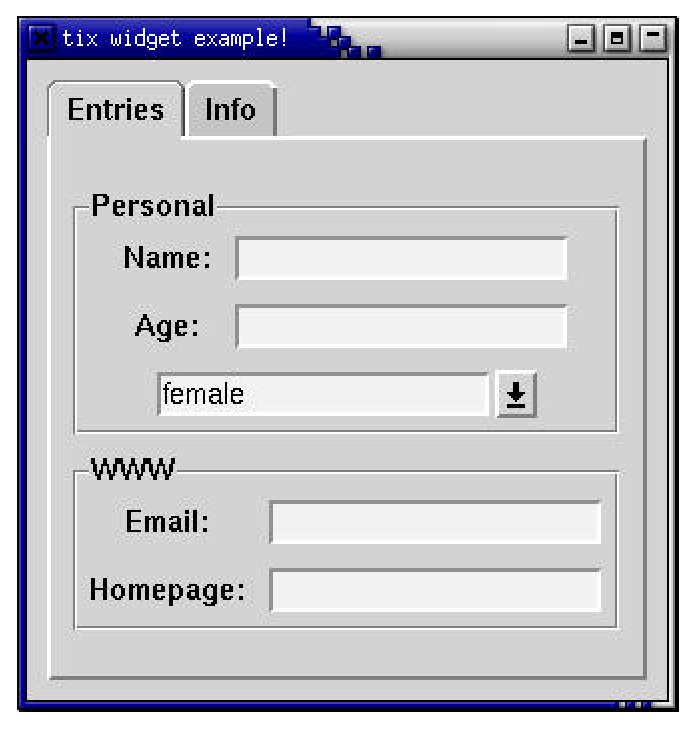
\includegraphics[width=7cm]{img/screenshot-tixwidgets}    
  \end{center}
  \caption{Tix Widgets}
  \label{fig:tix-widgets}
\end{wrapfigure}

To find out whether the \HTk program is currently running under a Tix
wish, use the function \texttt{isTixAvailable:: IO Bool}; a return
value \texttt{True} indicates Tix.

Here is an overview over the Tix widgets encapsulated by \HTk:

\begin{itemize}
\item The class \texttt{HasTooltip}, instantiated by all widgets,
  allows tooltips: text which is attached to the widget, and appears
  in a wee yellow box if the mouse hovers over the widget for a short
  while. Personally, I find this sort of thing immensely helpful.

\item A \emph{paned window} is a window divided into vertical or
  horizontal panes, which can be resized by the user. A well-known 
  example of this is Netscape's mail interface, or
  Adobe's acrobat reader, where you can change the size of the pane on
  the left (the mailboxes or the bookmarks) by grabbing the dividing
  line and moving it horizontally. For its usage, see
  \href{PanedWindow.html}{\texttt{PanedWindow}} and the example
  \texttt{MainPanedWindow.hs} in \texttt{htk/examples/tix}.

\item A \href{NoteBook.html}{note book} has a number of pages
  with tabs on top. It displays one page at a time, selected by the
  tab. The pages are represented by the type \texttt{NoteBookPage},
  which is an instance of the \texttt{Container} class, so you can
  pack widgets into them.

\item A \href{LabelFrame.html}{\texttt{LabelFrame}} is a frame with a
  label; useful for grouping information together. 

\item A \href{ComboBox.html}{combo box} is a combination of an entry
  and a list box, and as such has a value. Used much like list boxes,
  but with not quite as versatile selection schemes. 
\end{itemize}

Fig.~\ref{fig:tix-widgets} shows notebooks, labelled frames and a combo
box. 

There are many more Tix widgets, but we have found not all of them as
immediately useful as the ones above. Feel free to encapsulate more
(it should not be too hard). However, if you want to use Tix' tree
widgets, consider using the tree list from the toolkit (see below),
which is much nicer.

\section{The Toolkit}

\label{sec:toolkit}

The toolkit contains a number of so-called \emph{mega-widgets} and
\emph{dialog windows}. Mega-widgets are are widgets which are implemented in
Haskell rather than Tcl/Tk, and a dialog is a window querying the user
for information. We just mention these here, without explaining them
in detail, and show some screen shots. For most of them, their usage
is pretty obvious.

The examples mentioned below can be found in \texttt{htk/examples/toolkit}.

\subsection{Dialog Windows}

\begin{figure}[htbp]
  \begin{center}      
    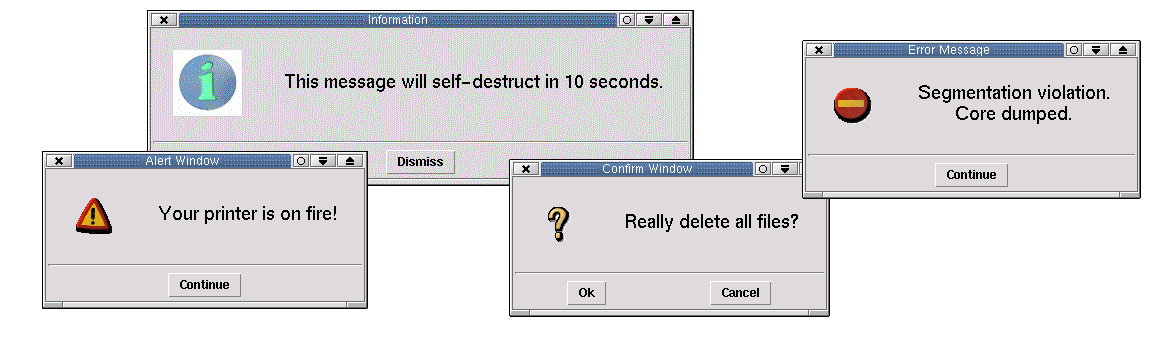
\includegraphics[width=\textwidth]{img/screenshot-dialogs}
    \caption{Dialog windows: alert, information, confirmation and error}
    \label{fig:dialogs}
  \end{center}
\end{figure}

The module \texttt{ModalDialog} builds  modal dialogue
(see Sect.~\ref{ssec:focus}) with toplevels (see
Sect.~\ref{ssec:focus}). The module \texttt{DialogWin} contains an
abstraction for dialogue windows, and built on top of that, frequently
used windows, such as alert, information, confirmation windows and
windows, and much more (Fig.~\ref{fig:dialogs}). See the example in
\texttt{Maindialog.hs}.


The module \texttt{FileDialog} implements a dialog query for a file
name while browsing the directory. The file dialog is vaguely in the
style of GTK+, with directories on the left and files on the
right. See the example in \texttt{Mainfiledialog.hs}, and the
screenshot in Fig.~\ref{fig:toolkit}.

\subsection{Mega-Widgets}

\begin{figure}[htbp]
   \begin{center}
     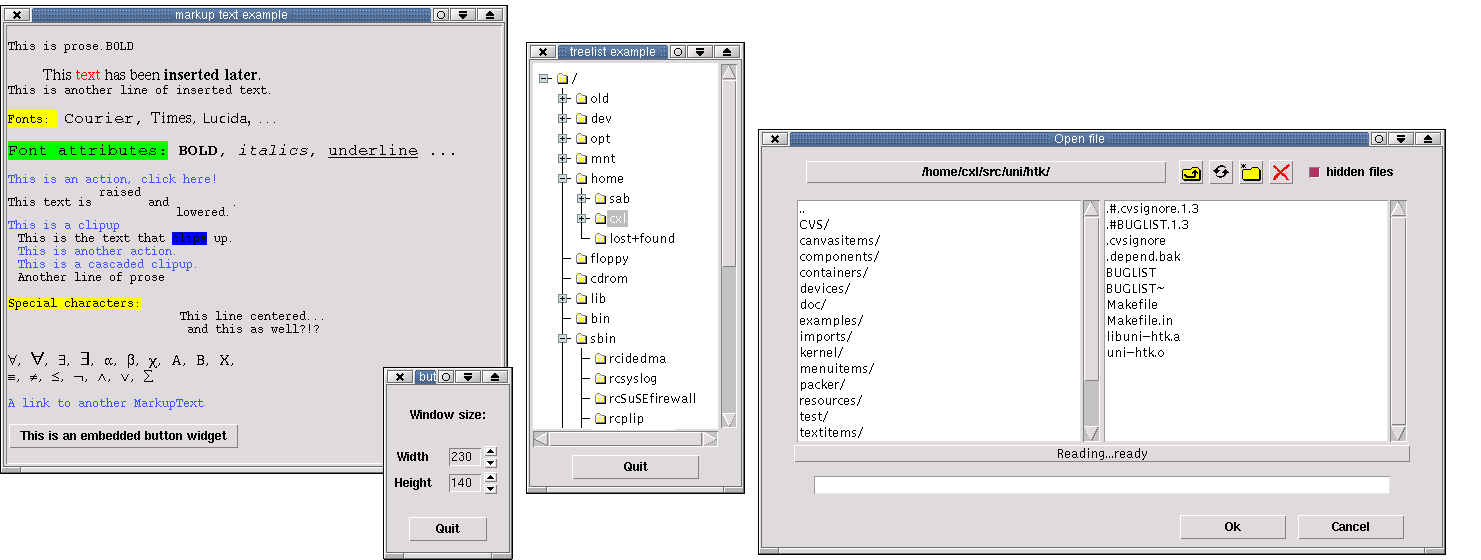
\includegraphics[width=\textwidth]{img/screenshot-toolkit}
     \caption{Toolkit components: Markup text, spin buttons, tree lists and a file dialog.}
     \label{fig:toolkit}
   \end{center}
\end{figure}

  The module \texttt{MarkupText} provides an easier, more abstract
  and flexible way of filling an editor with markup text. For example,
  you can simply write 
\begin{xcode}
 [prose "This is ", bold [prose "BOLD"], 
  prose " and ", bgcolour [prose "yellow."]]
\end{xcode}
 without needing to count the indices for the text tags
 manually. Hypertext, embedded widgets, mathematical symbols and much
 more are also supported. See also the example in \texttt{Mainmarkup.hs}.

  A \texttt{SpinButton} is a entry with two arrows which can
  increment or decrement the entry's value. See the example in
  \texttt{Mainspinbutton.hs}.
  
  A \texttt{TreeList} is a graphical representation of a tree
  structure. It allows subtrees to be hidden or shown. One popular use
  of this is to display the file system (see example
  \texttt{Maintreelist.hs}), but the possibilities are manyfold.

  The module \texttt{LogWin} implements a log window, a scrolled
  toplevel in which text is displayed, to which the program can
  append. The user can clear the whole text, or save it to a file. 

\subsection{Notepads and GenGUI}
  
  The \texttt{Notepad} is a canvas which displays \emph{items}. An
  item is given by the class \texttt{CItem}; it has a name and an
  icon. The notepad lets the user arrange the icons by dragging them
  around, and allows drag-and-drop between items.

  The generic \texttt{GenGUI} interface allows the visualisation
  of items which are arranged in a hierarchical structure. It uses a
  tree list to display the hierarchy, a notepad to display all items,
  and an editor to display a single item selectable by
  double-clicking. See the examples in \texttt{htk/examples/gengui}.

\subsection{Forms and Menus}

\label{ssec:forms-menus}

  The module \texttt{SimpleForm} implements forms in a simple, but
  typed manner. Roughly spoken, a form consists of pairs of a label
  and an entry, radio button, menu or other widget. The possible
  values entered by the user can be sanity-checked with so-called
  guards. See the example in \texttt{Mainsimpleform.hs}.

  The module \texttt{MenuType} gives an abstract (and rather more
  user-friendly way) of describing menus. It does not support radio
  buttons yet, but potentially you might want to use to build menus
  rather than Tk's slightly convoluted way (remember
  Sect.~\ref{sec:menues}). \texttt{HtkMenu} implements
  these for \texttt{HTk} (i.e. \texttt{MenuType} are the types, and
  \texttt{HTk} menu the implementation); see the example in
  \texttt{Mainsimplemenu.hs}.

\subsection{Small Mega-Widgets}

These are small but rather useful mega-widgets. We just mention them
briefly: 

  \begin{itemize}
  \item A \texttt{ScrollBox} is a scrollable widget inside a box scroll
    bars attached.
  \item A \texttt{Separator} is a frame with relief and borderwidth,
    to optically separate widgets.
  \item A \texttt{SelectBox} is a container for a group of buttons,
    one of which can be nominated as default button.
  \item An \texttt{IconBar} is a bar containing a row of buttons
    (ideally of the same size showing an image, but this is not
    enforced.) 
  \end{itemize}



\bibliography{intro}
\bibliographystyle{plain}

\newpage{}
\appendix{}

\input{MainhsMines.lhs}



\end{document}

%%% Local Variables: 
%%% mode: latex
%%% TeX-master: t
%%% End: 
